%% bare_conf.tex
%% V1.4b
%% 2015/08/26
%% by Michael Shell
%% See:
%% http://www.michaelshell.org/
%% for current contact information.
%%
%% This is a skeleton file demonstrating the use of IEEEtran.cls
%% (requires IEEEtran.cls version 1.8b or later) with an IEEE
%% conference paper.
%%
%% Support sites:
%% http://www.michaelshell.org/tex/ieeetran/
%% http://www.ctan.org/pkg/ieeetran
%% and
%% http://www.ieee.org/

%%*************************************************************************
%% Legal Notice:
%% This code is offered as-is without any warranty either expressed or
%% implied; without even the implied warranty of MERCHANTABILITY or
%% FITNESS FOR A PARTICULAR PURPOSE! 
%% User assumes all risk.
%% In no event shall the IEEE or any contributor to this code be liable for
%% any damages or losses, including, but not limited to, incidental,
%% consequential, or any other damages, resulting from the use or misuse
%% of any information contained here.
%%
%% All comments are the opinions of their respective authors and are not
%% necessarily endorsed by the IEEE.
%%
%% This work is distributed under the LaTeX Project Public License (LPPL)
%% ( http://www.latex-project.org/ ) version 1.3, and may be freely used,
%% distributed and modified. A copy of the LPPL, version 1.3, is included
%% in the base LaTeX documentation of all distributions of LaTeX released
%% 2003/12/01 or later.
%% Retain all contribution notices and credits.
%% ** Modified files should be clearly indicated as such, including  **
%% ** renaming them and changing author support contact information. **
%%*************************************************************************


% *** Authors should verify (and, if needed, correct) their LaTeX system  ***
% *** with the testflow diagnostic prior to trusting their LaTeX platform ***
% *** with production work. The IEEE's font choices and paper sizes can   ***
% *** trigger bugs that do not appear when using other class files.       ***                          ***
% The testflow support page is at:
% http://www.michaelshell.org/tex/testflow/



\documentclass[conference,a4paper]{IEEEtran}
% Some Computer Society conferences also require the compsoc mode option,
% but others use the standard conference format.
%
% If IEEEtran.cls has not been installed into the LaTeX system files,
% manually specify the path to it like:
% \documentclass[conference]{../sty/IEEEtran}


% Some very useful LaTeX packages include:
% (uncomment the ones you want to load)


% *** MISC UTILITY PACKAGES ***
%
%\usepackage{ifpdf}
% Heiko Oberdiek's ifpdf.sty is very useful if you need conditional
% compilation based on whether the output is pdf or dvi.
% usage:
% \ifpdf
%   % pdf code
% \else
%   % dvi code
% \fi
% The latest version of ifpdf.sty can be obtained from:
% http://www.ctan.org/pkg/ifpdf
% Also, note that IEEEtran.cls V1.7 and later provides a builtin
% \ifCLASSINFOpdf conditional that works the same way.
% When switching from latex to pdflatex and vice-versa, the compiler may
% have to be run twice to clear warning/error messages.
\usepackage{xcolor}
\usepackage{balance}


% *** CITATION PACKAGES ***
%
%\usepackage{cite}
% cite.sty was written by Donald Arseneau
% V1.6 and later of IEEEtran pre-defines the format of the cite.sty package
% \cite{} output to follow that of the IEEE. Loading the cite package will
% result in citation numbers being automatically sorted and properly
% "compressed/ranged". e.g., [1], [9], [2], [7], [5], [6] without using
% cite.sty will become [1], [2], [5]--[7], [9] using cite.sty. cite.sty's
% \cite will automatically add leading space, if needed. Use cite.sty's
% noadjust option (cite.sty V3.8 and later) if you want to turn this off
% such as if a citation ever needs to be enclosed in parenthesis.
% cite.sty is already installed on most LaTeX systems. Be sure and use
% version 5.0 (2009-03-20) and later if using hyperref.sty.
% The latest version can be obtained at:
% http://www.ctan.org/pkg/cite
% The documentation is contained in the cite.sty file itself.


% *** GRAPHICS RELATED PACKAGES ***
%
\ifCLASSINFOpdf
\usepackage[pdftex]{graphicx}
% declare the path(s) where your graphic files are
% \graphicspath{{../pdf/}{../jpeg/}}
% and their extensions so you won't have to specify these with
% every instance of \includegraphics
% \DeclareGraphicsExtensions{.pdf,.jpeg,.png}
\else
% or other class option (dvipsone, dvipdf, if not using dvips). graphicx
% will default to the driver specified in the system graphics.cfg if no
% driver is specified.
\usepackage[dvips]{graphicx}
% declare the path(s) where your graphic files are
% \graphicspath{{../eps/}}
% and their extensions so you won't have to specify these with
% every instance of \includegraphics
% \DeclareGraphicsExtensions{.eps}
\fi
% graphicx was written by David Carlisle and Sebastian Rahtz. It is
% required if you want graphics, photos, etc. graphicx.sty is already
% installed on most LaTeX systems. The latest version and documentation
% can be obtained at: 
% http://www.ctan.org/pkg/graphicx
% Another good source of documentation is "Using Imported Graphics in
% LaTeX2e" by Keith Reckdahl which can be found at:
% http://www.ctan.org/pkg/epslatex
%
% latex, and pdflatex in dvi mode, support graphics in encapsulated
% postscript (.eps) format. pdflatex in pdf mode supports graphics
% in .pdf, .jpeg, .png and .mps (metapost) formats. Users should ensure
% that all non-photo figures use a vector format (.eps, .pdf, .mps) and
% not a bitmapped formats (.jpeg, .png). The IEEE frowns on bitmapped formats
% which can result in "jaggedy"/blurry rendering of lines and letters as
% well as large increases in file sizes.
%
% You can find documentation about the pdfTeX application at:
% http://www.tug.org/applications/pdftex


% *** MATH PACKAGES ***
%
\usepackage{amsmath}
% A popular package from the American Mathematical Society that provides
% many useful and powerful commands for dealing with mathematics.
%
% Note that the amsmath package sets \interdisplaylinepenalty to 10000
% thus preventing page breaks from occurring within multiline equations. Use:
%\interdisplaylinepenalty=2500
% after loading amsmath to restore such page breaks as IEEEtran.cls normally
% does. amsmath.sty is already installed on most LaTeX systems. The latest
% version and documentation can be obtained at:
% http://www.ctan.org/pkg/amsmath


% *** SPECIALIZED LIST PACKAGES ***
%
\usepackage{algorithmic}
% algorithmic.sty was written by Peter Williams and Rogerio Brito.
% This package provides an algorithmic environment fo describing algorithms.
% You can use the algorithmic environment in-text or within a figure
% environment to provide for a floating algorithm. Do NOT use the algorithm
% floating environment provided by algorithm.sty (by the same authors) or
% algorithm2e.sty (by Christophe Fiorio) as the IEEE does not use dedicated
% algorithm float types and packages that provide these will not provide
% correct IEEE style captions. The latest version and documentation of
% algorithmic.sty can be obtained at:
% http://www.ctan.org/pkg/algorithms
% Also of interest may be the (relatively newer and more customizable)
% algorithmicx.sty package by Szasz Janos:
% http://www.ctan.org/pkg/algorithmicx


% *** ALIGNMENT PACKAGES ***
%
%\usepackage{array}
% Frank Mittelbach's and David Carlisle's array.sty patches and improves
% the standard LaTeX2e array and tabular environments to provide better
% appearance and additional user controls. As the default LaTeX2e table
% generation code is lacking to the point of almost being broken with
% respect to the quality of the end results, all users are strongly
% advised to use an enhanced (at the very least that provided by array.sty)
% set of table tools. array.sty is already installed on most systems. The
% latest version and documentation can be obtained at:
% http://www.ctan.org/pkg/array


% IEEEtran contains the IEEEeqnarray family of commands that can be used to
% generate multiline equations as well as matrices, tables, etc., of high
% quality.


% *** SUBFIGURE PACKAGES ***
\ifCLASSOPTIONcompsoc
\usepackage[caption=false,font=normalsize,labelfont=sf,textfont=sf]{subfig}
\else
\usepackage[caption=false,font=footnotesize]{subfig}
\fi
% subfig.sty, written by Steven Douglas Cochran, is the modern replacement
% for subfigure.sty, the latter of which is no longer maintained and is
% incompatible with some LaTeX packages including fixltx2e. However,
% subfig.sty requires and automatically loads Axel Sommerfeldt's caption.sty
% which will override IEEEtran.cls' handling of captions and this will result
% in non-IEEE style figure/table captions. To prevent this problem, be sure
% and invoke subfig.sty's "caption=false" package option (available since
% subfig.sty version 1.3, 2005/06/28) as this is will preserve IEEEtran.cls
% handling of captions.
% Note that the Computer Society format requires a larger sans serif font
% than the serif footnote size font used in traditional IEEE formatting
% and thus the need to invoke different subfig.sty package options depending
% on whether compsoc mode has been enabled.
%
% The latest version and documentation of subfig.sty can be obtained at:
% http://www.ctan.org/pkg/subfig


% *** FLOAT PACKAGES ***
%
%\usepackage{fixltx2e}
% fixltx2e, the successor to the earlier fix2col.sty, was written by
% Frank Mittelbach and David Carlisle. This package corrects a few problems
% in the LaTeX2e kernel, the most notable of which is that in current
% LaTeX2e releases, the ordering of single and double column floats is not
% guaranteed to be preserved. Thus, an unpatched LaTeX2e can allow a
% single column figure to be placed prior to an earlier double column
% figure.
% Be aware that LaTeX2e kernels dated 2015 and later have fixltx2e.sty's
% corrections already built into the system in which case a warning will
% be issued if an attempt is made to load fixltx2e.sty as it is no longer
% needed.
% The latest version and documentation can be found at:
% http://www.ctan.org/pkg/fixltx2e


%\usepackage{stfloats}
% stfloats.sty was written by Sigitas Tolusis. This package gives LaTeX2e
% the ability to do double column floats at the bottom of the page as well
% as the top. (e.g., "\begin{figure*}[!b]" is not normally possible in
% LaTeX2e). It also provides a command:
%\fnbelowfloat
% to enable the placement of footnotes below bottom floats (the standard
% LaTeX2e kernel puts them above bottom floats). This is an invasive package
% which rewrites many portions of the LaTeX2e float routines. It may not work
% with other packages that modify the LaTeX2e float routines. The latest
% version and documentation can be obtained at:
% http://www.ctan.org/pkg/stfloats
% Do not use the stfloats baselinefloat ability as the IEEE does not allow
% \baselineskip to stretch. Authors submitting work to the IEEE should note
% that the IEEE rarely uses double column equations and that authors should try
% to avoid such use. Do not be tempted to use the cuted.sty or midfloat.sty
% packages (also by Sigitas Tolusis) as the IEEE does not format its papers in
% such ways.
% Do not attempt to use stfloats with fixltx2e as they are incompatible.
% Instead, use Morten Hogholm'a dblfloatfix which combines the features
% of both fixltx2e and stfloats:
%
% \usepackage{dblfloatfix}
% The latest version can be found at:
% http://www.ctan.org/pkg/dblfloatfix


% *** PDF, URL AND HYPERLINK PACKAGES ***
%
%\usepackage{url}
% url.sty was written by Donald Arseneau. It provides better support for
% handling and breaking URLs. url.sty is already installed on most LaTeX
% systems. The latest version and documentation can be obtained at:
% http://www.ctan.org/pkg/url
% Basically, \url{my_url_here}.


% *** Do not adjust lengths that control margins, column widths, etc. ***
% *** Do not use packages that alter fonts (such as pslatex).         ***
% There should be no need to do such things with IEEEtran.cls V1.6 and later.
% (Unless specifically asked to do so by the journal or conference you plan
% to submit to, of course. )


% correct bad hyphenation here
\hyphenation{op-tical net-works semi-conduc-tor}

\usepackage[utf8]{inputenc}
\usepackage[T1]{fontenc}
\usepackage{amssymb}
\usepackage{import}


\begin{document}
%
% paper title
% Titles are generally capitalized except for words such as a, an, and, as,
% at, but, by, for, in, nor, of, on, or, the, to and up, which are usually
% not capitalized unless they are the first or last word of the title.
% Linebreaks \\ can be used within to get better formatting as desired.
% Do not put math or special symbols in the title.
    \title{Nanosatellite SAR Preliminary System Design for New Zealand Maritime and Terrestrial Remote Sensing}

% author names and affiliations
% use a multiple column layout for up to three different
% affiliations
    \author{\IEEEauthorblockN{
        Simone Mencarelli\IEEEauthorrefmark{1},   % 1st author, 1st affiliations
        Andrew C. M. Austin\IEEEauthorrefmark{2},   % 2nd author, 2nd affiliations
        Michael J. Neve\IEEEauthorrefmark{3}    % 3rd author, 3rd affiliations
    }                                     % ...
    \\
    \IEEEauthorblockA{Department of Electrical, Computer, and Software Engineering, \\The University of Auckland, Auckland, New Zealand}
    \IEEEauthorblockA{\IEEEauthorrefmark{1}% 1st affiliations
    smen851@aucklanduni.ac.nz, \IEEEauthorrefmark{2}% 2nd affiliations
    a.austin@auckland.ac.nz, \IEEEauthorrefmark{3}% 3rd affiliations
    mj.neve@auckland.ac.nz}}

% conference papers do not typically use \thanks and this command
% is locked out in conference mode. If really needed, such as for
% the acknowledgment of grants, issue a \IEEEoverridecommandlockouts
% after \documentclass


% use for special paper notices
%\IEEEspecialpapernotice{(Invited Paper)}


% make the title area
    \maketitle

% As a general rule, do not put math, special symbols or citations
% in the abstract
    \begin{abstract}
        The potential of nanosatellite radar sensors for illegal fishing vessel detection in the coastal waters and imaging on the land of New Zealand is investigated.
        It was found that for a sensor in Low Earth Orbit at an altitude of 500~km, with an antenna compatible in width with the longest side of a 3-U CubeSat, i.e., 0.3~m and a length of 2~m and a peak transmitted power of 200~W; adequate detection performance can be obtained over a swath of up to 60~km at an incidence angle of 36° using an ambiguous acquisition mode.
        Alternative solutions for different looking angles, but smaller swaths are also found to be viable.
        A design method and the resulting imaging performance for a land non-ambiguous imaging mode are also presented.
    \end{abstract}

    \vskip0.5\baselineskip
    \begin{IEEEkeywords}
        radar, synthetic aperture, SAR, system design, nanosatellite.
    \end{IEEEkeywords}


% For peer review papers, you can put extra information on the cover
% page as needed:
% \ifCLASSOPTIONpeerreview
% \begin{center} \bfseries EDICS Category: 3-BBND \end{center}
% \fi
%
% For peerreview papers, this IEEEtran command inserts a page break and
% creates the second title. It will be ignored for other modes.
% \IEEEpeerreviewmaketitle


    \section{Introduction}
    \label{sec:intro}
    With the ability to produce high-resolution observations day and night in most meteorological conditions, Synthetic Aperture Radar (SAR) \cite{moreira_tutorial} make an excellent candidate for the observation of New Zealand's sea and land.
    One of the problems that would benefit from radar imaging is the monitoring of illegal, unreported, and unregulated fishing vessels in New Zealand's Exclusive Economic Zone (EEZ).
    The New Zealand EEZ has an area of approximately 4$\times 10^6$~km$^2$ \cite{NZEEZ}, which makes detecting such vessels challenging with current methods \cite{JAN}.
    In addition, a SAR satellite or constellation, capable of observing the ocean over a broad swath and high revisit time would be ideal for maximizing the probability of locating such vessels in remote areas.
    SAR sensors can also be employed to monitor terrestrial features.
    Given the coherent nature of SAR images, it is possible to produce multi-pass interferometric measurements to monitor, for example, land subsidence and deformation over time \cite{Interferometry}.
    % This is of particular interest to New Zealand given its volcanic and seismic regions \cite{Interferometry}.
    Being part of the Pacific Ring of Fire, this is of particular interest to New Zealand for the study of its volcanic and seismic regions.
    Furthermore, a nanosatellite SAR sensor constellation could have several advantages over current satellite platforms, given their lower cost and scalability.
    In particular, coverage of vast areas with near real-time revisit time could be achieved \cite{ReviewCubeSats}, making the employment of this kind of sensor especially suited to the applications mentioned above.\\
    In practice, a small-satellite SAR will have limitations due to the reduced size.
    Most notably, it would be limited in peak power, while the antenna would have to rely on some deployable structure, e.g., \cite{Annalisa}, and most likely be limited in size and choice of form factor.
    Besides implying a low gain, this also limits the options when choosing the imaging resolution and swath while avoiding ambiguities, and the so-called \emph{minimum antenna area constraint} \cite{curlander1991synthetic} cannot always be satisfied.\\
    Concerning the low power constraint, it was shown in \cite{JAN} that the ship detection problem can be addressed with low power.
    Moreover, given the absence of alternative solutions, even modest probabilities of detection would be acceptable for a nanosatellite sensor.
    Subsequent work \cite{DLRjournal} has shown that wide-swath low-power ship detection can be performed using a narrow and relatively long antenna by employing a high-resolution azimuthally ambiguous acquisition mode in which slow-time undersampled data is zero-filled and processed using the nominal Doppler Bandwidth $B_D$.
    Results from \cite{JAN, DLRjournal} showed that a higher imaging resolution is the key to ship detection in noisy images.
    At the same time, the azimuth ambiguities pose little concern given the sparse nature of target vessels in the open sea.
    In \cite{DLRjournal} a model (backed by actual X-Band data) is provided to compute the probability of detection $P_d$ of certain classes of ships given the image \emph{Noise Equivalent Sigma Zero} (NESZ), resolution and desired probability of false alarm $P_{fa}$.
    Alternatively, if the radar is used for applications other than ship detection, the image cannot be ambiguous in azimuth.
    In this regard, using a reduced processed Doppler Bandwidth $B_p \leq B_D$, as proposed in \cite{freeman2018design}, could help bring down the \emph{Azimuth Ambiguity to Signal Ratio} (AASR) to within acceptable levels.\\
    The study in \cite{DLRjournal} provides some initial considerations for the system design, however $P_d$ is computed only at the swath edges and broadside direction considering a margin over the peak antenna gain. Moreover no timing constraints (e.g. to avoid ambiguous nadir returns) are considered, and results are presented for a single looking angle.
    % !! Need to link this work into the gap that should have been identified in the previous paragraph… perhaps need to end the previous paragraph on the limitations of that approach… !! -acma
    This work proposes a method to design an X-Band, nano-satellite-compatible SAR system with the Primary objective of detecting ships in the NZ EEZ, using the ambiguous acquisition mode of \cite{DLRjournal}.
    The goal in this context is to find one or more valid system designs with a wide ground swath (to minimize the number of passages required to cover the NZ EEZ) and evaluate the system performance over a set of looking angles or broadside ground incidence angles $\eta_i$.
    As a refinement to \cite{DLRjournal}, the timing constraints and the effect of ground illumination tapering given by the antenna pattern and the problem geometry are included in the design process.
    As a secondary objective, the design is then adapted to provide an unambiguous acquisition mode for land imaging by changing the \emph{Pulse Repetition Frequency} (PRF) and $B_p$, and an initial evaluation of performance and limitations for this mode are presented.\\
    The analysis presented here will initially assess a potential nanosatellite system performance.
    To this end, some assumptions have to be made on the radar characteristics: The antenna is assumed to be 0.3~m (el.) x 2~m (az.).
    This is to make the smaller side compatible with a 3U-12U CubeSat's largest dimension, while it is assumed that the antenna can be mechanically deployed in azimuth.
    The 2~m dimension should be sufficient for ship detection \cite{DLRjournal} while still being mechanically feasible, e.g., using the structure proposed in \cite{Annalisa}.
    For simplicity, the aperture is considered uniformly illuminated with no phase tapering, resulting in a sinc-shaped 2-d gain pattern;
    to keep complexity to a minimum, a single phase center (and Transmit Receive Module) is assumed.\\
    The maximum RF peak power is set to 200~W; by comparison, this corresponds to 1/4 of the peak power of the micro-satellite SAR Strix-$\alpha$ from Synspective \cite{StriX-a} and should be feasible using RF off-the-shelf components.
    A large duty cycle is assumed to compensate for the low peak power, i.e., 25\%. The losses $L$ and noise figure $F$ of the receiver are conservatively set to $L+F = 10$~dB as in \cite{JAN}.
    The minimum ship size to be detected is assumed to be 30~m~x~7~m as in \cite{JAN}.
    The minimum ground target resolution for ship detection imaging is set to $\delta_{az}\delta_{r}=2~$m$^2$ as the spotlight images resolution used in \cite{DLRjournal}, for a conservative $P_d$ estimation.
    Additionally $P_{fa} = 10^{-6}$, which corresponds to less than 1 false alarm per EEZ area (using eq. 14 in \cite{DLRjournal}).\\
    The remainder of this paper is structured as follows: in Section \ref{sec:systemDesign}, a system design algorithm is presented for the ambiguous ship detection mode, and seven potential design candidates are characterized and discussed.
    In section \ref{sec:psi}, the design procedure is modified to find a design candidate suitable for terrestrial imaging, and the resulting predicted performance is discussed.
    Lastly some conclusions are provided in Section \ref{sec:conclusion}.

    \section{System Design}
    \label{sec:systemDesign}
    In Table \ref{tab:parameters}, the initial design assumptions from the considerations in Section \ref{sec:intro} are summarized.
    \begin{table}[h]
        \caption{System Parameters}
        \label{tab:parameters}
        \centering
        \begin{tabular}{|l|l|l|}
            \hline
            & \textbf{Symbol}                       & \textbf{Value}     \\ \hline
            Carrier Frequency          & $f_c$                                 & 10 GHz             \\ \hline
            Orbital height             & $h$                                   & 500 km             \\ \hline
            Antenna dimensions         & $W_a \times L_a$                      & 0.3 m $\times$ 2 m \\ \hline
            Peak Tx Power              & $P_{peak}$                            & 200 W              \\ \hline
            Losses + Noise Figure      & $L+F$                                 & 10 dB              \\ \hline
            Antenna Temperature        & $T_a$                                 & 300 K              \\ \hline
            Duty Cycle                 & $\delta$                              & 0.25               \\ \hline
            Resolution Area            & $A_{res}=\delta_{az}\delta_{r}$       & 2 m$^2$            \\ \hline
            Ship size                  & $A_{ship}$                            & 7 m $\times$ 30 m  \\ \hline
            Prob. of False Alarm       & $P_{fa}$                              & $1\times 10^{-6}$  \\ \hline
            Minimum Prob. of Detection & $P_{d_{min}}$ \rule[-1.1mm]{0mm}{1mm} & 0.5                \\ \hline
        \end{tabular}
    \end{table}
    The ship detection problem will benefit from a wide swath.
    However, the "useful" portion of the ground range that can be imaged will be limited by two factors: (i) The probability of detection variation over the ground range;
    and (ii) the timing constraint.
    The $P_d$ will mainly depend on the ground illumination given by the antenna pattern, and is therefore limited by the antenna elevation beamwidth.
    In regard to timing constraints, the PRF has to be low enough to "view" the desired ground swath, also considering the blind ranges given by the transmit events.
    Additionally, the pulse interval has to be chosen to avoid nadir returns, i.e., to minimize the possibility of having range ambiguities in the image.
    As a result, the set of "valid" ground range swath --- PRF pairs will be discrete, and the ground swath that the radar can observe will be defined by the PRF, the pulse duty cycle, and the \emph{order} of the pulses backscattered by the targets within the swath \cite{curlander1991synthetic}.
    This timing constraint is visually represented in Fig. \ref{fig:timingdiagram}, where the orange stripes represent the transmit events and the black lines the location of nadir interferences.
    It should be noted that the actual swath will be smaller than the distance between the edges of two consecutive transmit events because of the integration time for the range impulse compression, wich is not negligible for a $\delta$ this high.\\
    The $P_d$ as a function of the ground range, slant range, or $\eta$ angle, is computed from the equations in \cite{DLRjournal} for \emph{medium} ships (with length comprised between 25~m and 150~m), using the selected $P_{fa}$, the NESZ and the ground resolution area.
    The NESZ in this work is defined as
    \begin{equation}
        \text{NESZ} =\dfrac{128 \pi^3 r^4\ F L k T_a B_n\  \sin{\eta}\int_{B_p}\left| H(f_d) \right|^2\, df_d}{P_{av}\  \lambda^2\ G^2\ c\ B_p\ v_s}
        \label{eq:nesz}
    \end{equation}
    where $\lambda$ is the wavelength, $\eta$ is the incidence angle, $r$ is the distance between target and radar, $v_s$ is the average orbital speed of the satellite, $k$ is the Boltzmann constant, $c$ is the speed of light, $f_d$ is the Doppler shift, $B_n$ is the chirp (noise) bandwidth, and $G$ is the antenna peak gain.
    Lastly $|H(f_d)|$ is the amplitude of the Doppler (slow-time) compression filter designed to compensate for the azimuth antenna pattern tapering so that the azimuthal resolution $\delta_{az}\approx L_a/2$ is constant all over the swath.
    In contrast, the noise power will vary over the swath accordingly to $\int_{B_{p}}|H(f_d, \eta)|^2$, i.e., a function of the integrated antenna pattern inverse.
    A spherical earth geometry is assumed in all calculations;
    the incidence angle $\eta$, ground range $r_g$, and slant range $r$ are defined accordingly and related to each other.
    The incidence angle of the antenna broadside direction projected on ground (which will depend on the looking angle) is denoted as $\eta_i$.
    \begin{figure*}[t]
        \centering
        \subfloat[ ]{
            \begin{normalsize}
                \import{./}{tdfig.pdf_tex}
            \end{normalsize}
        %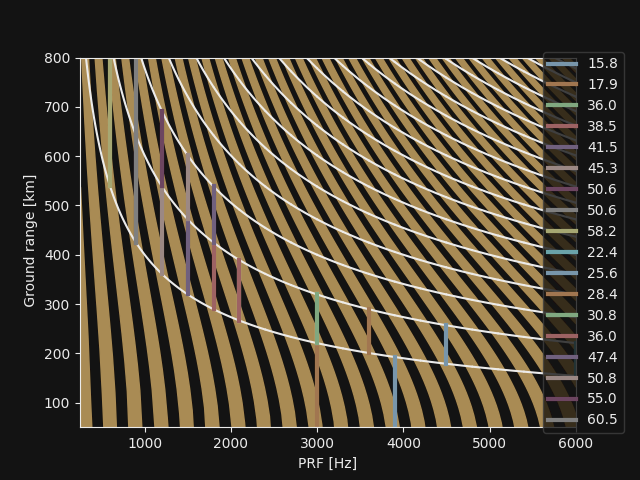
\includegraphics[width=0.8\columnwidth]{timingdiagram}%
            \label{fig:timingdiagram}}
        \hfil
        \subfloat[]{
            \begin{normalsize}
                \import{./}{pd.pdf_tex}
            \end{normalsize}
        %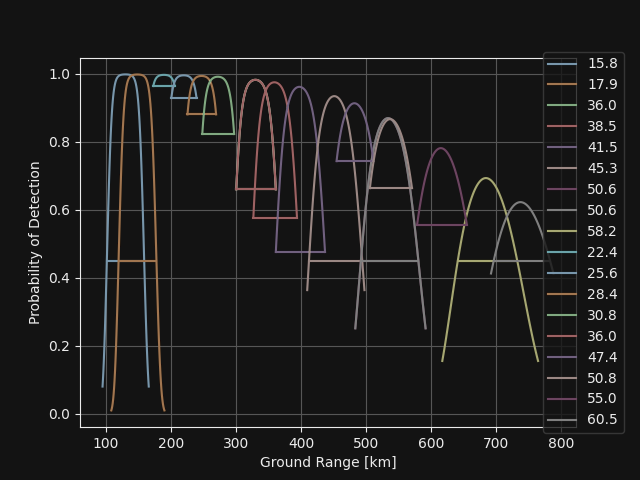
\includegraphics[width=.8\columnwidth]{probdect}%
            \label{fig:Probability of Detection}}
        \caption{The timing diagram (a) and the Probability of detection (b) for a selection of valid design candidates with different looking angles.}
        \label{fig:double column}
    \end{figure*}

    \subsection{Procedure}
    \label{subsec:procedure}
    To select the broadest possible ground swath while satisfying the timing constraints, the following design algorithm is proposed.\\
    An initial broadside incidence angle is set based on the ground portion to be observed;
    the procedure then tries to \emph{lock} to the closest valid timing diagram slot prioritizing the solution that provides the widest swath on Earth's surface.
    The output will be an incidence angle (different than the starting one) --- PRF pair that maximizes $P_d$ over the swath accordingly to the model described in Section \ref{sec:systemDesign}.
%    \begin{algorithmic}[1]
%        \STATE Set the initial radar looking angle from $\eta_i$.
%        \STATE \label{pt:band}Find the chirp bandwidth form $A_{res}$ using: $B_n = c L_a / (4 \sin{\eta_i} A_{res} )$
%        \STATE Compute the NESZ using \eqref{eq:nesz}
%        \STATE Compute $P_d$ from NESZ
%        \STATE \label{pt:swath1}Find the initial swath extremes $r_{1}$ and $r_{2}$ so that: $P_d(r_1) = P_d(r_1) = P_{d_{min}}$
%        \IF  {$(r_2 - r_1) \leq \left[r(\theta_i + \theta_{el}/2) - r(\theta_i + \theta_{el}/2) \right]$}
%        \STATE $r_{1,2} = r(\theta_i \pm \theta_{el}/2)$ ;to avoid range ambiguities
%        \ENDIF \label{pt:swath2}
%        \STATE \label{pt:PRI0}Find the initial $\text{PRI} = 2(r_2 - r_1) / \left[c (1-2\delta)\right]$
%        \STATE \label{pt:timingconstraint} Update the PRI using the closest valid timing diagram point (see Fig. \ref{fig:timingdiagram})
%        \STATE Update $r_{1,2}$ setting $r_{1} = (n + \delta)\text{PRI}\ c / 2 $  and\\ $r_2 = (n + 1 - \delta)\text{PRI}\ c / 2\; ;\ n\in \mathbb{N}$
%        \STATE Update $ B_n $ as in \ref{pt:band}: setting $\eta_i = [\eta(r_1) + \eta(r_2)] / 2$
%        \STATE Recenter the antenna i.e. find the $\eta_i$ angle so that $P_d(r_1) = P_d(r_2)$
%        \IF {The desired region of observation is within $r_{g_{1,2}}$}
%        \RETURN $\eta_i$, PRI, $r_{1,2}$
%        \ELSE
%        \STATE \label{pt:relaxed}Relax the constraint on swath, setting \\$r_{1,2} = r(\theta_i \pm \alpha\ \theta_{el}/2)\; ;\ 0< \alpha < 1 $
%        \STATE \textbf{goto} \ref{pt:PRI0}:
%        \ENDIF
%    \end{algorithmic}
    \begin{enumerate}
        \item Set the initial radar looking angle from $\eta_i$.
        \item \label{pt:band}Find the chirp bandwidth form $A_{res}$ using: $B_n = c L_a / (4 \sin{\eta_i} A_{res} )$
        \item Compute the NESZ using \eqref{eq:nesz}
        \item Compute $P_d$ from NESZ
        \item \label{pt:swath1}Find the initial swath extremes $r_{1}$ and $r_{2}$ so that: $P_d(r_1) = P_d(r_1) = P_{d_{min}}$
        \item \label{pt:swath2} \textbf{if} {$(r_2 - r_1) \leq \left[r(\theta_i + \theta_{el}/2) - r(\theta_i - \theta_{el}/2) \right]$}
        \begin{enumerate}
            \item $r_{1,2} = r(\theta_i \pm \theta_{el}/2)$ ;to avoid range ambiguities
        \end{enumerate}
        \item \label{pt:PRI0}Find the initial $\text{PRI} = 2(r_2 - r_1) / \left[c (1-2\delta)\right]$
        \label{pt:timingconstraint} Update the PRI using the closest valid timing diagram point (see Fig. \ref{fig:timingdiagram})
        \item Update $r_{1,2}$ setting $r_{1} = (n + \delta)\text{PRI}\ c / 2 $  and\\ $r_2 = (n + 1 - \delta)\text{PRI}\ c / 2\; ;\ n\in \mathbb{N}$
        \item Update $ B_n $ as in \ref{pt:band} setting $\eta_i = [\eta(r_1) + \eta(r_2)] / 2$
        \item Recenter the antenna i.e. find the $\eta_i$ angle so that $P_d(r_1) = P_d(r_2)$
        \item \textbf{if} {The desired region of observation is within $r_{g_{1,2}}$}
        \begin{enumerate}
            \item \textbf{return} $\eta_i$, PRI, $r_{1,2}$
        \end{enumerate}
        \item \textbf{else}
        \begin{enumerate}
            \item \label{pt:relaxed}Relax the constraint on swath, setting \\$r_{1,2} = r(\theta_i \pm \alpha\ \theta_{el}/2)\; ;\ 0< \alpha < 1 $
        \end{enumerate}
        \item repeat from step \ref{pt:PRI0}
    \end{enumerate}

    In the algorithm, PRI $=$ $1/$PRF is the Pulse Repetition Interval, $\theta_{el} \approx \lambda/W_a$ is the elevation antenna beamwidth, $\theta_i$ is the radar side-looking angle associated with the incidence angle and $n$ is the pulse order of the signal of interest.
    When computing the NESZ \eqref{eq:nesz} to find $P_d$, is assumed that $B_p = B_D$, where $B_D$ is the nominal Doppler bandwidth related to the azimuth antenna beamwidth i.e. $B_D \approx 2 v_s / L_a$.

    \subsection{Design examples}
    \label{subsec:analysis}
    The design procedure of section \ref{subsec:procedure} was iterated for different initial incidence angles, first only using the swath constraint from step \ref{pt:swath1} to \ref{pt:swath2}, then by slightly relaxing the swath constraint as per step \ref{pt:relaxed}.
    In this way, the design space can be mapped to see what happens if we want to image different parts of the swath and the trade-offs associated with different design solutions.\\
    Seven of the resulting design \emph{points} are selected.
    In Fig. \ref{fig:timingdiagram} the timing diagram is plotted with the design solutions displayed as colored pulse-to-pulse vertical lines, while the \emph{visible} swath (factoring in duty cycle and pulse compression) is marked by two `+'.
    Fig. \ref{fig:Probability of Detection} shows the $P_d$ variation over the swath for each design point.
    The horizontal lines in Fig. \ref{fig:Probability of Detection} mark the \emph{useful} ground swath $W_g$, i.e., the swath over which ships would be detected with a $P_d \geq P_{d_{min}}$.
    The $\eta_i$ values in the legend are the incidence angles of the resulting antenna broadside pointing direction for each solution.\\
    In Table \ref{tab:analysis}, some numerical values are reported for the same design points: the \emph{useful} ground swath, the chirp bandwidth to satisfy the ground resolution requirement (this is to be considered a minimum value requirement, an higher bandwidth is expected to produce better results as explained in \cite{DLRjournal}), and the \emph{undersampling} factor $B_D/$PRF, which, since we are considering an ambiguous acquisition mode in azimuth, is always larger than 1.
    Additionally, the Azimuth Ambiguity to Signal Ratio (AASR), defined as in \cite{curlander1991synthetic}, and computed using the along-track cut of the antenna pattern, is tabulated along with the peak value of the Range Ambiguity to Signal Ratio (RASR) within the useful swath, also defined as in \cite{curlander1991synthetic}, and computed using the elevation integrated antenna pattern.
    \begin{table}[t]
        \caption{Design examples results}
        \label{tab:analysis}
        \centering
        %\renewcommand{\arraystretch}{1}
        \large
        \resizebox{\columnwidth}{!}{
            \begin{tabular}{|l|l|l|l|l|l|l|l|}
                \hline
                Case no.                               & 1            & 2            & 3            & 4            & 5            & 6            & 7            \\\hline
                $\eta_i$\rule[0mm]{0mm}{3.1mm}         & 17.9$^\circ$ & 25.6$^\circ$ & 30.8$^\circ$ & 36.0$^\circ$ & 38.5$^\circ$ & 45.4$^\circ$ & 58.3$^\circ$ \\\hline
                $W_g$[km]\rule[0mm]{0mm}{3.1mm}        & 56.8         & 38.7         & 48.9         & 60.8         & 67.1         & 78.3         & 81.4         \\\hline
                $B_n$[MHz]\rule[0mm]{0mm}{3.1mm}       & 245.3        & 173.9        & 146.7        & 127.7        & 120.8        & 105.6        & 88.3         \\\hline
                $B_D/\text{PRF}$\rule[0mm]{0mm}{3.1mm} & 2.5          & 1.7          & 2.5          & 3.6          & 4.2          & 6.4          & 12.7         \\\hline
                AASR[dB]\rule[0mm]{0mm}{3.1mm}         & 2.3          & 1.9          & 3.4          & 4.5          & 4.2          & 6.7          & 12.6         \\\hline
                RASR[dB]\rule[0mm]{0mm}{3.1mm}         & -32.4        & -22.9        & -19.5        & -18.7        & -19.6        & -26.8        & -26.5        \\\hline
            \end{tabular}}
    \end{table}
    A note that has to be made regarding these results is the following: the $P_d$ model utilized here is based on data from observations made between a declared range of 22$^\circ$ to 40$^\circ$ for the incidence angle $\eta$.
    Some results slightly outside this boundary are reported for completeness.
    Still, in a final system design, only those within the above range should be considered without further studies on the characteristics of scatterers at those angles.\\
    The first observation from these results is that the swath width varies discontinuously when compared to $\eta_i$.
    This discontinuity follows from the fact that to avoid the first nadir return, the swath constraint has to be relaxed and the PRF increased;
    as a result, for $\eta_i$ between 22$^\circ$ and 35$^\circ$ (i.e., ground ranges approximately between 180--300 km), the achievable swath width is much smaller than for the design points with larger or smaller $\eta_i$.
    Second, it can be seen that the general trend for the peak $P_d$ is decreasing with the ground swath, which is to be expected given the increase in the slant range.\\
    The RASR level, as expected due to the low values for the PRF, is within acceptable levels for all the presented solutions.
    The AASR, as expected, is quite large, given the $B_D/\text{PRF}>1$; however, as explained in \cite{DLRjournal}, this is not a problem, for the replicas of the ship targets will be identifiable as ambiguities (and potentially exploited to increase $P_d$ using a more sophisticated detection algorithm), while the increased clutter noise due to azimuth ambiguities will not affect the detection performance significantly.
    Furthermore, the chirp bandwidth is kept between 100--200 MHz for most design points, even though an higher bandwidth will theoretically give better results, a nanosatellite might be limited in terms of downlink or storage capacity, therefore is good to have some margin (which could allow a longer azimuth strip to be imaged).
    % Overall, a wide enough set of solutions exist to cover different parts of the ground swath from the same orbit.\\
    If the looking angle can be chosen arbitrarily, a good design solution is the one for $\eta_i=36^\circ$ in Table \ref{tab:analysis} that provides a ground swath of 60.8~km while remaining within the 22$^\circ$--40$^\circ$ incidence angle range of validity over all the swath.
    By comparison, the fifth solution in Table \ref{tab:analysis} presents a wider swath, however, even if the broadside angle of incidence is within the validity range, the incidence angle of points in the far end of the swath exceed 40$^\circ$.
    Furthermore, the analysis was repeated to find a larger number of design points with incidence angles in the 22$^\circ$--40$^\circ$ range, and it was found that the parameters on the fourth solution of Table \ref{tab:analysis}, are still the ones providing the largest swath with $P_d>P_{d_{min}}$.
    Other valid solutions exist, but will cover a narrower ground swath.
    Still, these can be used whenever a specific portion of ground not covered by the radar pointing the antenna to $\eta_i=36^\circ$, has to be imaged.

    \section{Unambiguous imaging mode}
    \label{sec:psi}
    A canonical SAR system for land imaging, given the specified antenna width $W_a$ would require an antenna much longer than the one in Table \ref{tab:parameters}.
    Given the PRF and the duty cycle are properly chosen to keep the range ambiguities (i.e., RASR) below an acceptable level within the imaged swath;
    if the ratio between PRF and nominal Doppler bandwidth $B_d$ is between 1 and 2, the azimuth ambiguities (AASR) can be reduced by choosing a processed Doppler bandwidth $B_p < B_D$  \cite{freeman2018design}.
    On the other hand, a reduction of $B_d$ comes at the expense of a lower azimuth resolution.\\
    By inspection of Table \ref{tab:analysis} we can see that only one design candidate presents an undersampling ratio lower than 2.
    Expanding the analysis it was noted that design points with lower $B_D/\text{PRF}$ present a narrower swath for similar looking angles, this is due to the higher PRF.
    These two considerations suggest that it is indeed possible to obtain a non-ambiguous image from the same satellite.
    Instead of using the same PRF and $\eta_i$ of the above "valid" solution, we can try to further reduce the swath width to increase the PRF (at the expense of an higher RASR).
    Furthermore, given the transmit power is already low, a narrower looking angle is preferable (and will also tend to have a higher PRF).\\
    A method is proposed in section \ref{subsec:psiproc} to select the optimal system parameters:

    \subsection{Procedure}
    \label{subsec:psiproc}
    The design procedure can be simplified as follows to satisfy land imaging requirements:
    \begin{enumerate}
        \item Set the initial radar looking angle from $\eta_i$.
        \item Set the chirp bandwidth
        \item Select the ground range extremes as $r_{1,2} = r(\theta_i \pm \theta_{el}/2)$
        \item Find the initial $\text{PRI} = 2(r_2 - r_1) / c $ ;without considering the duty cycle
        \item Update the PRI using the closest valid timing diagram point (see Fig. \ref{fig:timingdiagram})
        \item Update $r_{1,2}$ setting $r_{1} = (n + \delta)\text{PRI}\ c / 2 $  and\\ $r_2 = (n + 1 - \delta)\text{PRI}\ c / 2\; ;\ n\in \mathbb{N}$
        \item Recenter the antenna i.e. find the $\eta_i$ angle so that $\text{NESZ}(r_1) = \text{NESZ}(r_2)$
        \item Set $B_p = B_D$
        \item find $B_p$ so that AASR$=$AASR$_{max}$ \label{pt:optim}
        \item \textbf{return} $\eta_i$, PRI, $r_{1,2},\  B_p$
    \end{enumerate}
    In point \ref{pt:optim} it can be assumed that AASR is monotonically decreasing with $B_p$ \cite{freeman2018design}, however is not guaranteed that a solution exists for an arbitrarily low AASR$_{max}$.

    \subsection{Example}
    \label{subsec:psiexample}
    \begin{figure}[ht]
        \centering
        \begin{normalsize}
            \import{./}{psifig.pdf_tex}
        \end{normalsize}
        %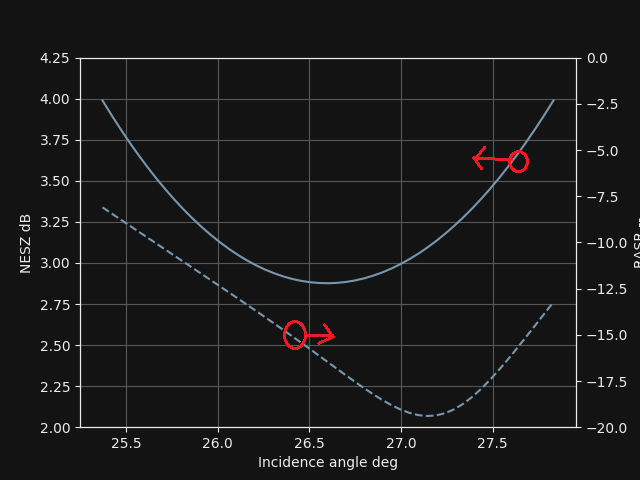
\includegraphics[width=0.8\columnwidth]{psi}
        \caption{Unambiguous mode predicted NESZ and RASR}
        \label{fig:eucap}
    \end{figure}
    The system parameters for one resulting design candidate are shown in Table \ref{tab:psi}.
    Other parameters such as antenna size, power, frequency etc. are the same of Table \ref{tab:parameters}.
    The ground swath $W_g$, is defined as the visible swath (i.e., limited by PRF, duty cycle, and pulse compression).
    \begin{table}[h]
        \caption{Land Imaging System Design}
        \label{tab:psi}
        \centering
        \begin{tabular}{|l|l|}
            \hline
            $\eta_i$      & 26.8$^\circ$ \\ \hline
            $W_g$         & 24.3 km      \\ \hline
            $B_n$         & 200 MHz      \\ \hline
            $B_p/B_D$     & 0.75         \\ \hline
            $\delta_{az}$ & 1.3 m        \\ \hline
            AASR          & -14 dB       \\ \hline
        \end{tabular}
    \end{table}
    In Fig. \ref{fig:eucap}, the NESZ and The RASR for the design example are plotted over the ground swath.
    The final image resolution and the swath width resulting from the design procedure are in line with larger and more expensive SAR platforms, with the azimuth resolution only slightly larger than the one used for ship detection.
    However, the NESZ and RASR values are extremely poor by canonical standards \cite{curlander1991synthetic}.
    As a result a single satellite with this acquisition mode with these system constraints, will only be able to "see" very bright targets or artificial corner reflectors (that still might be sufficient for some very specific interferometric applications).
    More useful results might be obtained if multilooking techniques \cite{curlander1991synthetic,moreira_tutorial} are employed, by repeatedly passing over the scene with the same sensor or using multiple identical nanosatellite sensors.
    Furthermore, some increase in performance might be obtained slightly increasing the duty cycle (at the expense of a narrower swath), the antenna size or the transmitted power.


    \section{Conclusion}
    \label{sec:conclusion}
    The potential of a nanosatellite radar mission for the monitoring of New Zealand's Exclusive Economic Zone and land was explored in this work.
    A design methodology for the ship detection problem, based on recent SAR techniques that enable the detection of ships with small antenna and low power transmitters, was proposed to include the effect of antenna pattern tapering and timing constraints.
    It was found that an antenna of 0.3~m x 2~m in size and a peak RF radiated power of 200W are sufficient to detect potential illegal fishing vessel that might operate in New Zealand's territorial waters.
    A set of valid system parameter candidates was presented for incidence angles between 22$^\circ$ and 40$^\circ$ finding that ground swaths between 38.7~km and 60.8~km can be covered with adequate detection performance and a low level of range ambiguities (RASR<-18~dB).
    The dependency between ground swath and looking angle was characterized showing that the swath width cannot be chosen to be arbitrarily large by reducing the antenna aperture size in elevation.
    The optimal looking angle for wide swath imaging, given the system constraints was selected accordingly.
    Additionally, a design procedure to use the same system for land imaging was proposed and a design example presented and characterized finding that an azimuth ground resolution of 1.2~m and swath of 24.3~km can be obtained, but with low single acquisition dynamic range performance i.e., NESZ~>~2.8~dB and RASR$\approx$10~dB.\\

% use section* for acknowledgment
%    \section*{Acknowledgment}


% trigger a \newpage just before the given reference
% number - used to balance the columns on the last page
% adjust value as needed - may need to be readjusted if
% the document is modified later
% \IEEEtriggeratref{7}
% The "triggered" command can be changed if desired:
% \IEEEtriggercmd{\enlargethispage{-20cm}}

% references section

% can use a bibliography generated by BibTeX as a .bbl file
% BibTeX documentation can be easily obtained at:
% http://mirror.ctan.org/biblio/bibtex/contrib/doc/
% The IEEEtran BibTeX style support page is at:
% http://www.michaelshell.org/tex/ieeetran/bibtex/
%\bibliographystyle{IEEEtran}
% argument is your BibTeX string definitions and bibliography database(s)
%\bibliography{IEEEabrv,../bib/paper}
%
% <OR> manually copy in the resultant .bbl file
% set second argument of \begin to the number of references
% (used to reserve space for the reference number labels box)
    \bibliographystyle{IEEEtran}
    \bibliography{bibliograpy}

    \color{red}
% add name of last editor and increase the v count
    %draft v2 Simone
% that's all folks
\end{document}


